\documentclass{standalone}
\usepackage{tikz}
\usepackage{url}
\usetikzlibrary{shapes.geometric, arrows.meta, positioning, fit}

\begin{document}
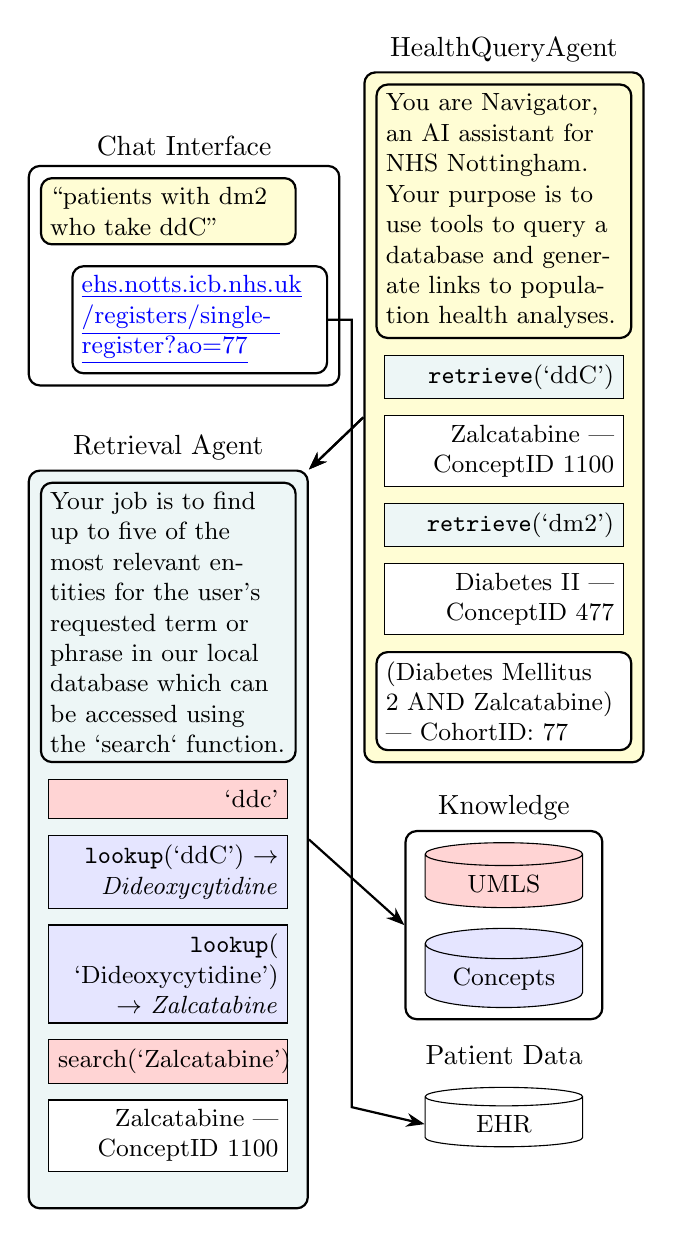
\begin{tikzpicture}[
    node distance=2mm, % vertical spacing between nodes
    innerbox/.style={rectangle, draw, solid, thick, rounded corners, minimum width=1.5cm, minimum height=0.5cm, align=left, text width=3cm, font=\small},
    outerbox/.style={rectangle, draw, thick, rounded corners, minimum width=3.5cm, minimum height=2cm, inner sep=4pt},
    knowledgebox/.style={outerbox, minimum width=2.5cm, minimum height=0.5cm},
    promptbox/.style={innerbox, fill=yellow!17},
    databox/.style={rectangle, draw, solid, minimum width=2.8cm, text width=2.8cm, minimum height=0.5cm, align=left, font=\small, fill=white, align=right},
    retrievetool/.style={rectangle, draw, solid, minimum width=2.8cm, text width=2.8cm, minimum height=0.5cm, align=left, font=\small, fill=teal!7, align=right},
    searchtool/.style={rectangle, draw, solid, minimum width=2.8cm, text width=2.8cm, minimum height=0.5cm, align=left, font=\small, fill=red!17, align=right},
    umlstool/.style={rectangle, draw, solid, minimum width=2.8cm, text width=2.8cm, minimum height=0.5cm, align=left, font=\small, fill=blue!10, align=right},
    linkbox/.style={innerbox, fill=yellow!17},
    arrow/.style={-Stealth, thick},
    data/.style={cylinder, font=\small}
]

% User Interface components
\node[innerbox, fill=yellow!17] (request) {``patients with dm2 who take ddC''};
\node[innerbox, below=0.25cm of request, xshift=4mm] (response) {
\textcolor{blue}{
\underline{ehs.notts.icb.nhs.uk}
\underline{/registers/single- }
\underline{register?ao=77}}
};

% Processing components
\node[innerbox, right=1cm of request] (prompt) {You are Navigator, an AI assistant for NHS Nottingham. Your purpose is to use tools to query a database and generate links to population health analyses.};
\node[retrievetool, below=of prompt] (search1)  {retrieve(`ddC')};
\node[databox, below=of search1] (result1) {Zalcatabine | ConceptID 1100};
\node[retrievetool, below=of result1] (search2) {\texttt{retrieve}(`dm2')};
\node[databox, below=of search2] (result2) {Diabetes II | ConceptID 477};
\node[innerbox, below=of result2] (backend) {(Diabetes Mellitus 2 AND Zalcatabine) | CohortID: 77};


% Retrieval Sub-agent 
\node[innerbox, below=3cm of request] (retrieval0) {Your job is to find up to five of the most relevant entities for the user's requested term or phrase in our local database which can be accessed using the `search` function.};
\node[searchtool, below=of retrieval0] (retrieval1) {`ddc'};
\node[umlstool, below=of retrieval1] (retrieval2) {\texttt{lookup}(`ddC') $\rightarrow$ \textit{Dideoxycytidine}};
\node[umlstool, below=of retrieval2] (retrieval3) {\texttt{lookup}( \\ `Dideoxycytidine') $\rightarrow$ \textit{Zalcatabine}};
\node[searchtool, below=of retrieval3] (retrieval4) {search(`Zalcatabine')};
\node[databox, below=of retrieval4] (retrieval5) {Zalcatabine | ConceptID = 11002};

% Data-Layer
% \node[database, below=3cm of backend] (db) {EHR};
% \node[database, base right=1cm of db.base] (umls) {UMLS};

% Grouping boxes
\node[outerbox, fit=(request) (response), label=above:Chat Interface] (interface) {};
\node[outerbox, fit=(prompt) (search1) (result1) (search2) (result2) (backend), label=above:HealthQueryAgent, fill=yellow!17] (processing) {};
\node[outerbox, fit=(retrieval0) (retrieval1) (retrieval2) (retrieval3) (retrieval4) (retrieval5), fill=teal!7, label=above:Retrieval Agent] (retrieval) {};

%%% DUPLICATES FOR PLOTTING OVER THE BACKGROUND BOXES -- KEEP IN SYNC %%%
\node[innerbox, below=3cm of request] (aretrieval0) {Your job is to find up to five of the most relevant entities for the user's requested term or phrase in our local database which can be accessed using the `search` function.};
\node[searchtool, below=of retrieval0] (aretrieval1) {`ddc'};
\node[umlstool, below=of retrieval1] (aretrieval2) {\texttt{lookup}(`ddC') $\rightarrow$ \textit{Dideoxycytidine}};
\node[umlstool, below=of retrieval2] (aretrieval3) {\texttt{lookup}( \\ `Dideoxycytidine') $\rightarrow$ \textit{Zalcatabine}};
\node[searchtool, below=of retrieval3] (aretrieval4) {search(`Zalcatabine')};
\node[databox, below=of retrieval4] (aretrieval5) {Zalcatabine | ConceptID 1100};

\node[innerbox, right=1cm of request] (aprompt) {You are Navigator, an AI assistant for NHS Nottingham. Your purpose is to use tools to query a database and generate links to population health analyses.};
\node[retrievetool, below=of prompt] (asearch1)  {\texttt{retrieve}(`ddC')};
\node[databox, below=of search1] (aresult1) {Zalcatabine | ConceptID 1100};
\node[retrievetool, below=of result1] (asearch2) {\texttt{retrieve}(`dm2')};
\node[databox, below=of search2] (aresult2) {Diabetes II | ConceptID 477};
\node[innerbox, below=of result2, fill=white] (abackend) {(Diabetes Mellitus 2 AND Zalcatabine) | CohortID: 77};


%%%%%%%%%%%%%%%%%%%%%%%%%%%%%%%%%%%%%%%%%%%%%%%%%%%%%%%%%%%%%%%%%%%%%%%%%%


% Define both database nodes
\node[data, aspect=0.25, draw, shape border rotate=90, minimum height=1, minimum width=2cm, below=1cm of processing,  fill=red!17] (umls) {UMLS};
\node[data, aspect=0.25, draw, shape border rotate=90, minimum height=1, minimum width=2cm, below=0.25cm of umls, fill=blue!10] (concept) {Concepts};

% Patient Data
\node[data, aspect=0.25, draw, shape border rotate=90, minimum height=1, minimum width=2cm, below=1cm of concept] (ehr) {EHR};

% Then the data layer grouping box that fits both
\node[knowledgebox, fit=(umls) (concept), label=above:Knowledge] (data) {};

% TODO make invis box
\node[knowledgebox, draw=none, fit=(ehr), label=above:Patient Data] (patientdata) {};


% Arrows
% \draw[arrow] (ehr.north) |- ++(-3.125, 1) |- (response.east);
% \draw[arrow] (retrieval2.east) -- (umls.west);
% \draw[arrow] (retrieval3.east) -- (umls.west);
% \draw[arrow] (retrieval4.east) |- ++(3, 0) -- (ehr.south);
% \draw[arrow] (backend.south) -- (ehr.north);

\draw[arrow] (processing.west) -- (retrieval.north east);
% TODO: offset the second arrow:
\draw[arrow] (processing.west) -- (retrieval.north east);

% sub-agent dashed-lines
\draw[arrow] (retrieval.east) -- (data.west);

\draw[arrow] (response.east) --  ++(3mm,0) -- ++(0,-10cm) -- (ehr.west);

\end{tikzpicture}
\end{document}

